10. $\cfrac{(x+2)(x+3)}{(x+1)^2}\geqslant0.$ Применив метод интервалов, найдём ответ: $x\in(-\infty;-3]\cup[-2;-1)\cup(-1;+\infty).$
\begin{figure}[ht!]
\center{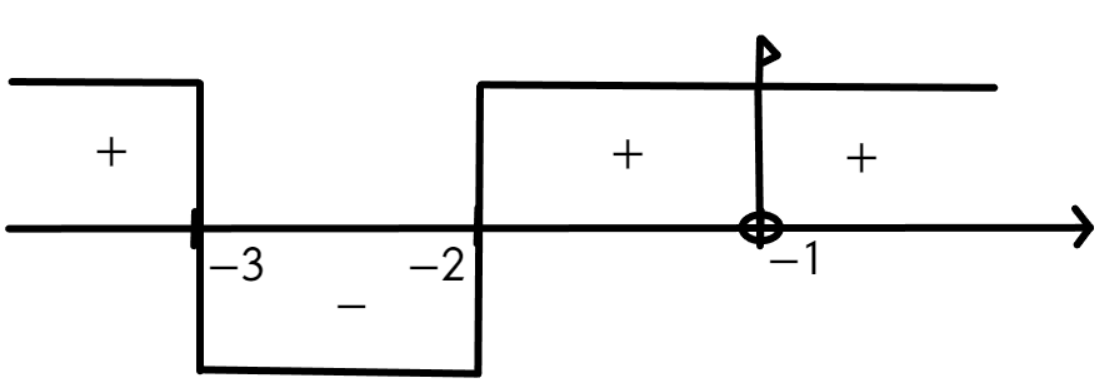
\includegraphics[scale=0.35]{ner9-10.png}}
\end{figure}\\
